\PassOptionsToPackage{unicode=true}{hyperref} % options for packages loaded elsewhere
\PassOptionsToPackage{hyphens}{url}
%
\documentclass[ignorenonframetext,]{beamer}
\usepackage{pgfpages}
\setbeamertemplate{caption}[numbered]
\setbeamertemplate{caption label separator}{: }
\setbeamercolor{caption name}{fg=normal text.fg}
\beamertemplatenavigationsymbolsempty
% Prevent slide breaks in the middle of a paragraph:
\widowpenalties 1 10000
\raggedbottom
\setbeamertemplate{part page}{
\centering
\begin{beamercolorbox}[sep=16pt,center]{part title}
  \usebeamerfont{part title}\insertpart\par
\end{beamercolorbox}
}
\setbeamertemplate{section page}{
\centering
\begin{beamercolorbox}[sep=12pt,center]{part title}
  \usebeamerfont{section title}\insertsection\par
\end{beamercolorbox}
}
\setbeamertemplate{subsection page}{
\centering
\begin{beamercolorbox}[sep=8pt,center]{part title}
  \usebeamerfont{subsection title}\insertsubsection\par
\end{beamercolorbox}
}
\AtBeginPart{
  \frame{\partpage}
}
\AtBeginSection{
  \ifbibliography
  \else
    \frame{\sectionpage}
  \fi
}
\AtBeginSubsection{
  \frame{\subsectionpage}
}
\usepackage{lmodern}
\usepackage{amssymb,amsmath}
\usepackage{ifxetex,ifluatex}
\usepackage{fixltx2e} % provides \textsubscript
\ifnum 0\ifxetex 1\fi\ifluatex 1\fi=0 % if pdftex
  \usepackage[T1]{fontenc}
  \usepackage[utf8]{inputenc}
  \usepackage{textcomp} % provides euro and other symbols
\else % if luatex or xelatex
  \usepackage{unicode-math}
  \defaultfontfeatures{Ligatures=TeX,Scale=MatchLowercase}
\fi
% use upquote if available, for straight quotes in verbatim environments
\IfFileExists{upquote.sty}{\usepackage{upquote}}{}
% use microtype if available
\IfFileExists{microtype.sty}{%
\usepackage[]{microtype}
\UseMicrotypeSet[protrusion]{basicmath} % disable protrusion for tt fonts
}{}
\IfFileExists{parskip.sty}{%
\usepackage{parskip}
}{% else
\setlength{\parindent}{0pt}
\setlength{\parskip}{6pt plus 2pt minus 1pt}
}
\usepackage{hyperref}
\hypersetup{
            pdftitle={Marketing Science with R},
            pdfauthor={TokyoR \#78 Kien Knot(きぬいと; @0\_u0)},
            pdfborder={0 0 0},
            breaklinks=true}
\urlstyle{same}  % don't use monospace font for urls
\newif\ifbibliography
\usepackage{color}
\usepackage{fancyvrb}
\newcommand{\VerbBar}{|}
\newcommand{\VERB}{\Verb[commandchars=\\\{\}]}
\DefineVerbatimEnvironment{Highlighting}{Verbatim}{commandchars=\\\{\}}
% Add ',fontsize=\small' for more characters per line
\usepackage{framed}
\definecolor{shadecolor}{RGB}{248,248,248}
\newenvironment{Shaded}{\begin{snugshade}}{\end{snugshade}}
\newcommand{\AlertTok}[1]{\textcolor[rgb]{0.94,0.16,0.16}{#1}}
\newcommand{\AnnotationTok}[1]{\textcolor[rgb]{0.56,0.35,0.01}{\textbf{\textit{#1}}}}
\newcommand{\AttributeTok}[1]{\textcolor[rgb]{0.77,0.63,0.00}{#1}}
\newcommand{\BaseNTok}[1]{\textcolor[rgb]{0.00,0.00,0.81}{#1}}
\newcommand{\BuiltInTok}[1]{#1}
\newcommand{\CharTok}[1]{\textcolor[rgb]{0.31,0.60,0.02}{#1}}
\newcommand{\CommentTok}[1]{\textcolor[rgb]{0.56,0.35,0.01}{\textit{#1}}}
\newcommand{\CommentVarTok}[1]{\textcolor[rgb]{0.56,0.35,0.01}{\textbf{\textit{#1}}}}
\newcommand{\ConstantTok}[1]{\textcolor[rgb]{0.00,0.00,0.00}{#1}}
\newcommand{\ControlFlowTok}[1]{\textcolor[rgb]{0.13,0.29,0.53}{\textbf{#1}}}
\newcommand{\DataTypeTok}[1]{\textcolor[rgb]{0.13,0.29,0.53}{#1}}
\newcommand{\DecValTok}[1]{\textcolor[rgb]{0.00,0.00,0.81}{#1}}
\newcommand{\DocumentationTok}[1]{\textcolor[rgb]{0.56,0.35,0.01}{\textbf{\textit{#1}}}}
\newcommand{\ErrorTok}[1]{\textcolor[rgb]{0.64,0.00,0.00}{\textbf{#1}}}
\newcommand{\ExtensionTok}[1]{#1}
\newcommand{\FloatTok}[1]{\textcolor[rgb]{0.00,0.00,0.81}{#1}}
\newcommand{\FunctionTok}[1]{\textcolor[rgb]{0.00,0.00,0.00}{#1}}
\newcommand{\ImportTok}[1]{#1}
\newcommand{\InformationTok}[1]{\textcolor[rgb]{0.56,0.35,0.01}{\textbf{\textit{#1}}}}
\newcommand{\KeywordTok}[1]{\textcolor[rgb]{0.13,0.29,0.53}{\textbf{#1}}}
\newcommand{\NormalTok}[1]{#1}
\newcommand{\OperatorTok}[1]{\textcolor[rgb]{0.81,0.36,0.00}{\textbf{#1}}}
\newcommand{\OtherTok}[1]{\textcolor[rgb]{0.56,0.35,0.01}{#1}}
\newcommand{\PreprocessorTok}[1]{\textcolor[rgb]{0.56,0.35,0.01}{\textit{#1}}}
\newcommand{\RegionMarkerTok}[1]{#1}
\newcommand{\SpecialCharTok}[1]{\textcolor[rgb]{0.00,0.00,0.00}{#1}}
\newcommand{\SpecialStringTok}[1]{\textcolor[rgb]{0.31,0.60,0.02}{#1}}
\newcommand{\StringTok}[1]{\textcolor[rgb]{0.31,0.60,0.02}{#1}}
\newcommand{\VariableTok}[1]{\textcolor[rgb]{0.00,0.00,0.00}{#1}}
\newcommand{\VerbatimStringTok}[1]{\textcolor[rgb]{0.31,0.60,0.02}{#1}}
\newcommand{\WarningTok}[1]{\textcolor[rgb]{0.56,0.35,0.01}{\textbf{\textit{#1}}}}
\usepackage{graphicx,grffile}
\makeatletter
\def\maxwidth{\ifdim\Gin@nat@width>\linewidth\linewidth\else\Gin@nat@width\fi}
\def\maxheight{\ifdim\Gin@nat@height>\textheight\textheight\else\Gin@nat@height\fi}
\makeatother
% Scale images if necessary, so that they will not overflow the page
% margins by default, and it is still possible to overwrite the defaults
% using explicit options in \includegraphics[width, height, ...]{}
\setkeys{Gin}{width=\maxwidth,height=\maxheight,keepaspectratio}
\setlength{\emergencystretch}{3em}  % prevent overfull lines
\providecommand{\tightlist}{%
  \setlength{\itemsep}{0pt}\setlength{\parskip}{0pt}}
\setcounter{secnumdepth}{0}

% set default figure placement to htbp
\makeatletter
\def\fps@figure{htbp}
\makeatother


\title{Marketing Science with R}
\author{TokyoR \#78 Kien Knot(きぬいと; @0\_u0)}
\date{2019/5/25}

\begin{document}
\frame{\titlepage}

\begin{frame}{自己紹介}

\begin{itemize}
\tightlist
\item
  労働者階級2年目

  \begin{itemize}
  \tightlist
  \item
    マーケティング系調査屋さんのアナリスト

    \begin{itemize}
    \tightlist
    \item
      兼アナリスト候補のヘッドハンター
    \item
      兼部署内作業環境改善係
    \item
      兼広報担当
    \end{itemize}
  \end{itemize}
\item
  最近の出来事

  \begin{itemize}
  \tightlist
  \item
    転職しないことにした

    \begin{itemize}
    \tightlist
    \item
      キャリアなんもわからん問題でバズってしまった
    \item
      なお今もなんもわからん模様
    \end{itemize}
  \item
    OSをUbuntuに変えたらMSOffice使えないじゃない\ldots{}\ldots{}
  \end{itemize}
\end{itemize}

\end{frame}

\begin{frame}{宣伝}

\begin{itemize}
\tightlist
\item
  Statistician-jaのDiscordをつくりました

  \begin{itemize}
  \tightlist
  \item
    「数理統計学」をやっていくサーバ

    \begin{itemize}
    \tightlist
    \item
      「10人くらいかなあ」
    \end{itemize}
  \end{itemize}
\item
  今では300人超えてきた

  \begin{itemize}
  \tightlist
  \item
    FF外からいっぱい来た
  \item
    界隈のドンからも反響があった
  \end{itemize}
\end{itemize}

\end{frame}

\begin{frame}{宣伝}
\protect\hypertarget{-1}{}

\includegraphics{./.picture/thinker.jpeg}

\end{frame}

\begin{frame}[fragile]{嬉しい悲鳴}

\begin{itemize}
\tightlist
\item
  PythonとかRとかではなく「数理統計」のお勉強をやろう

  \begin{itemize}
  \tightlist
  \item
    \texttt{lm(y\textasciitilde{}.,\ data\ =\ dat)}の裏のロジックをつかもう
  \item
    理論は廃れないのでみんなで理解しよう
  \end{itemize}
\item
  目標は統計検定1級に合格することなど
\item
  \url{https://discord.gg/Nq75Smp}にアクセス!

  \begin{itemize}
  \tightlist
  \item
    Meetupとかも構想中です。
  \item
    運営の仕方とか教えてほしい
  \end{itemize}
\end{itemize}

\end{frame}

\begin{frame}{今日のお話}

\begin{itemize}
\tightlist
\item
  「Rって非Tech系企業でどう使われているんですか?」なお話

  \begin{itemize}
  \tightlist
  \item
    R: エンジニアじゃない人も割と使ってる
  \item
    故に「バージョン管理」とかよく分かってないことも\ldots{}\ldots{}

    \begin{itemize}
    \tightlist
    \item
      最近社内で\href{https://speakerdeck.com/s_uryu/rstudio-for-team}{Uribo先生の資料}を紹介しました
    \end{itemize}
  \end{itemize}
\item
  マーケティング・リサーチ業界でのお話

  \begin{itemize}
  \tightlist
  \item
    偏見があります
  \end{itemize}
\item
  R要素は?

  \begin{itemize}
  \tightlist
  \item
    これがRmarkdownでできている
  \item
    それで十分じゃないか\ldots{}\ldots{}?
  \item
    ioslideの無骨さいい\ldots{}\ldots{}
  \end{itemize}
\end{itemize}

\end{frame}

\section{「マーケティング」って何?}

\begin{frame}[fragile]{実際に聞いてみたい}

\begin{itemize}
\tightlist
\item
  Q.「マーケティングってなんだと思いますか?」
\end{itemize}

\begin{verbatim}
## Warning in axis(if (horiz) 2 else 1, at = at.l, labels = names.arg, lty =
## axis.lty, : 'mbcsToSbcs' 中の '1.よくわからない' で変換に失敗: <e3> をドッ
## トで置き換えました
\end{verbatim}

\begin{verbatim}
## Warning in axis(if (horiz) 2 else 1, at = at.l, labels = names.arg, lty =
## axis.lty, : 'mbcsToSbcs' 中の '1.よくわからない' で変換に失敗: <82> をドッ
## トで置き換えました
\end{verbatim}

\begin{verbatim}
## Warning in axis(if (horiz) 2 else 1, at = at.l, labels = names.arg, lty =
## axis.lty, : 'mbcsToSbcs' 中の '1.よくわからない' で変換に失敗: <88> をドッ
## トで置き換えました
\end{verbatim}

\begin{verbatim}
## Warning in axis(if (horiz) 2 else 1, at = at.l, labels = names.arg, lty =
## axis.lty, : 'mbcsToSbcs' 中の '1.よくわからない' で変換に失敗: <e3> をドッ
## トで置き換えました
\end{verbatim}

\begin{verbatim}
## Warning in axis(if (horiz) 2 else 1, at = at.l, labels = names.arg, lty =
## axis.lty, : 'mbcsToSbcs' 中の '1.よくわからない' で変換に失敗: <81> をドッ
## トで置き換えました
\end{verbatim}

\begin{verbatim}
## Warning in axis(if (horiz) 2 else 1, at = at.l, labels = names.arg, lty =
## axis.lty, : 'mbcsToSbcs' 中の '1.よくわからない' で変換に失敗: <8f> をドッ
## トで置き換えました
\end{verbatim}

\begin{verbatim}
## Warning in axis(if (horiz) 2 else 1, at = at.l, labels = names.arg, lty =
## axis.lty, : 'mbcsToSbcs' 中の '1.よくわからない' で変換に失敗: <e3> をドッ
## トで置き換えました
\end{verbatim}

\begin{verbatim}
## Warning in axis(if (horiz) 2 else 1, at = at.l, labels = names.arg, lty =
## axis.lty, : 'mbcsToSbcs' 中の '1.よくわからない' で変換に失敗: <82> をドッ
## トで置き換えました
\end{verbatim}

\begin{verbatim}
## Warning in axis(if (horiz) 2 else 1, at = at.l, labels = names.arg, lty =
## axis.lty, : 'mbcsToSbcs' 中の '1.よくわからない' で変換に失敗: <8f> をドッ
## トで置き換えました
\end{verbatim}

\begin{verbatim}
## Warning in axis(if (horiz) 2 else 1, at = at.l, labels = names.arg, lty =
## axis.lty, : 'mbcsToSbcs' 中の '1.よくわからない' で変換に失敗: <e3> をドッ
## トで置き換えました
\end{verbatim}

\begin{verbatim}
## Warning in axis(if (horiz) 2 else 1, at = at.l, labels = names.arg, lty =
## axis.lty, : 'mbcsToSbcs' 中の '1.よくわからない' で変換に失敗: <81> をドッ
## トで置き換えました
\end{verbatim}

\begin{verbatim}
## Warning in axis(if (horiz) 2 else 1, at = at.l, labels = names.arg, lty =
## axis.lty, : 'mbcsToSbcs' 中の '1.よくわからない' で変換に失敗: <8b> をドッ
## トで置き換えました
\end{verbatim}

\begin{verbatim}
## Warning in axis(if (horiz) 2 else 1, at = at.l, labels = names.arg, lty =
## axis.lty, : 'mbcsToSbcs' 中の '1.よくわからない' で変換に失敗: <e3> をドッ
## トで置き換えました
\end{verbatim}

\begin{verbatim}
## Warning in axis(if (horiz) 2 else 1, at = at.l, labels = names.arg, lty =
## axis.lty, : 'mbcsToSbcs' 中の '1.よくわからない' で変換に失敗: <82> をドッ
## トで置き換えました
\end{verbatim}

\begin{verbatim}
## Warning in axis(if (horiz) 2 else 1, at = at.l, labels = names.arg, lty =
## axis.lty, : 'mbcsToSbcs' 中の '1.よくわからない' で変換に失敗: <89> をドッ
## トで置き換えました
\end{verbatim}

\begin{verbatim}
## Warning in axis(if (horiz) 2 else 1, at = at.l, labels = names.arg, lty =
## axis.lty, : 'mbcsToSbcs' 中の '1.よくわからない' で変換に失敗: <e3> をドッ
## トで置き換えました
\end{verbatim}

\begin{verbatim}
## Warning in axis(if (horiz) 2 else 1, at = at.l, labels = names.arg, lty =
## axis.lty, : 'mbcsToSbcs' 中の '1.よくわからない' で変換に失敗: <81> をドッ
## トで置き換えました
\end{verbatim}

\begin{verbatim}
## Warning in axis(if (horiz) 2 else 1, at = at.l, labels = names.arg, lty =
## axis.lty, : 'mbcsToSbcs' 中の '1.よくわからない' で変換に失敗: <aa> をドッ
## トで置き換えました
\end{verbatim}

\begin{verbatim}
## Warning in axis(if (horiz) 2 else 1, at = at.l, labels = names.arg, lty =
## axis.lty, : 'mbcsToSbcs' 中の '1.よくわからない' で変換に失敗: <e3> をドッ
## トで置き換えました
\end{verbatim}

\begin{verbatim}
## Warning in axis(if (horiz) 2 else 1, at = at.l, labels = names.arg, lty =
## axis.lty, : 'mbcsToSbcs' 中の '1.よくわからない' で変換に失敗: <81> をドッ
## トで置き換えました
\end{verbatim}

\begin{verbatim}
## Warning in axis(if (horiz) 2 else 1, at = at.l, labels = names.arg, lty =
## axis.lty, : 'mbcsToSbcs' 中の '1.よくわからない' で変換に失敗: <84> をドッ
## トで置き換えました
\end{verbatim}

\begin{verbatim}
## Warning in axis(if (horiz) 2 else 1, at = at.l, labels = names.arg, lty =
## axis.lty, : 'mbcsToSbcs' 中の '1.よくわからない' で変換に失敗: <e3> をドッ
## トで置き換えました
\end{verbatim}

\begin{verbatim}
## Warning in axis(if (horiz) 2 else 1, at = at.l, labels = names.arg, lty =
## axis.lty, : 'mbcsToSbcs' 中の '1.よくわからない' で変換に失敗: <82> をドッ
## トで置き換えました
\end{verbatim}

\begin{verbatim}
## Warning in axis(if (horiz) 2 else 1, at = at.l, labels = names.arg, lty =
## axis.lty, : 'mbcsToSbcs' 中の '1.よくわからない' で変換に失敗: <88> をドッ
## トで置き換えました
\end{verbatim}

\begin{verbatim}
## Warning in axis(if (horiz) 2 else 1, at = at.l, labels = names.arg, lty =
## axis.lty, : 'mbcsToSbcs' 中の '1.よくわからない' で変換に失敗: <e3> をドッ
## トで置き換えました
\end{verbatim}

\begin{verbatim}
## Warning in axis(if (horiz) 2 else 1, at = at.l, labels = names.arg, lty =
## axis.lty, : 'mbcsToSbcs' 中の '1.よくわからない' で変換に失敗: <81> をドッ
## トで置き換えました
\end{verbatim}

\begin{verbatim}
## Warning in axis(if (horiz) 2 else 1, at = at.l, labels = names.arg, lty =
## axis.lty, : 'mbcsToSbcs' 中の '1.よくわからない' で変換に失敗: <8f> をドッ
## トで置き換えました
\end{verbatim}

\begin{verbatim}
## Warning in axis(if (horiz) 2 else 1, at = at.l, labels = names.arg, lty =
## axis.lty, : 'mbcsToSbcs' 中の '1.よくわからない' で変換に失敗: <e3> をドッ
## トで置き換えました
\end{verbatim}

\begin{verbatim}
## Warning in axis(if (horiz) 2 else 1, at = at.l, labels = names.arg, lty =
## axis.lty, : 'mbcsToSbcs' 中の '1.よくわからない' で変換に失敗: <82> をドッ
## トで置き換えました
\end{verbatim}

\begin{verbatim}
## Warning in axis(if (horiz) 2 else 1, at = at.l, labels = names.arg, lty =
## axis.lty, : 'mbcsToSbcs' 中の '1.よくわからない' で変換に失敗: <8f> をドッ
## トで置き換えました
\end{verbatim}

\begin{verbatim}
## Warning in axis(if (horiz) 2 else 1, at = at.l, labels = names.arg, lty =
## axis.lty, : 'mbcsToSbcs' 中の '1.よくわからない' で変換に失敗: <e3> をドッ
## トで置き換えました
\end{verbatim}

\begin{verbatim}
## Warning in axis(if (horiz) 2 else 1, at = at.l, labels = names.arg, lty =
## axis.lty, : 'mbcsToSbcs' 中の '1.よくわからない' で変換に失敗: <81> をドッ
## トで置き換えました
\end{verbatim}

\begin{verbatim}
## Warning in axis(if (horiz) 2 else 1, at = at.l, labels = names.arg, lty =
## axis.lty, : 'mbcsToSbcs' 中の '1.よくわからない' で変換に失敗: <8b> をドッ
## トで置き換えました
\end{verbatim}

\begin{verbatim}
## Warning in axis(if (horiz) 2 else 1, at = at.l, labels = names.arg, lty =
## axis.lty, : 'mbcsToSbcs' 中の '1.よくわからない' で変換に失敗: <e3> をドッ
## トで置き換えました
\end{verbatim}

\begin{verbatim}
## Warning in axis(if (horiz) 2 else 1, at = at.l, labels = names.arg, lty =
## axis.lty, : 'mbcsToSbcs' 中の '1.よくわからない' で変換に失敗: <82> をドッ
## トで置き換えました
\end{verbatim}

\begin{verbatim}
## Warning in axis(if (horiz) 2 else 1, at = at.l, labels = names.arg, lty =
## axis.lty, : 'mbcsToSbcs' 中の '1.よくわからない' で変換に失敗: <89> をドッ
## トで置き換えました
\end{verbatim}

\begin{verbatim}
## Warning in axis(if (horiz) 2 else 1, at = at.l, labels = names.arg, lty =
## axis.lty, : 'mbcsToSbcs' 中の '1.よくわからない' で変換に失敗: <e3> をドッ
## トで置き換えました
\end{verbatim}

\begin{verbatim}
## Warning in axis(if (horiz) 2 else 1, at = at.l, labels = names.arg, lty =
## axis.lty, : 'mbcsToSbcs' 中の '1.よくわからない' で変換に失敗: <81> をドッ
## トで置き換えました
\end{verbatim}

\begin{verbatim}
## Warning in axis(if (horiz) 2 else 1, at = at.l, labels = names.arg, lty =
## axis.lty, : 'mbcsToSbcs' 中の '1.よくわからない' で変換に失敗: <aa> をドッ
## トで置き換えました
\end{verbatim}

\begin{verbatim}
## Warning in axis(if (horiz) 2 else 1, at = at.l, labels = names.arg, lty =
## axis.lty, : 'mbcsToSbcs' 中の '1.よくわからない' で変換に失敗: <e3> をドッ
## トで置き換えました
\end{verbatim}

\begin{verbatim}
## Warning in axis(if (horiz) 2 else 1, at = at.l, labels = names.arg, lty =
## axis.lty, : 'mbcsToSbcs' 中の '1.よくわからない' で変換に失敗: <81> をドッ
## トで置き換えました
\end{verbatim}

\begin{verbatim}
## Warning in axis(if (horiz) 2 else 1, at = at.l, labels = names.arg, lty =
## axis.lty, : 'mbcsToSbcs' 中の '1.よくわからない' で変換に失敗: <84> をドッ
## トで置き換えました
\end{verbatim}

\begin{verbatim}
## Warning in axis(if (horiz) 2 else 1, at = at.l, labels = names.arg, lty =
## axis.lty, : 'mbcsToSbcs' 中の '2.意識高い' で変換に失敗: <e6> をドットで置
## き換えました
\end{verbatim}

\begin{verbatim}
## Warning in axis(if (horiz) 2 else 1, at = at.l, labels = names.arg, lty =
## axis.lty, : 'mbcsToSbcs' 中の '2.意識高い' で変換に失敗: <84> をドットで置
## き換えました
\end{verbatim}

\begin{verbatim}
## Warning in axis(if (horiz) 2 else 1, at = at.l, labels = names.arg, lty =
## axis.lty, : 'mbcsToSbcs' 中の '2.意識高い' で変換に失敗: <8f> をドットで置
## き換えました
\end{verbatim}

\begin{verbatim}
## Warning in axis(if (horiz) 2 else 1, at = at.l, labels = names.arg, lty =
## axis.lty, : 'mbcsToSbcs' 中の '2.意識高い' で変換に失敗: <e8> をドットで置
## き換えました
\end{verbatim}

\begin{verbatim}
## Warning in axis(if (horiz) 2 else 1, at = at.l, labels = names.arg, lty =
## axis.lty, : 'mbcsToSbcs' 中の '2.意識高い' で変換に失敗: <ad> をドットで置
## き換えました
\end{verbatim}

\begin{verbatim}
## Warning in axis(if (horiz) 2 else 1, at = at.l, labels = names.arg, lty =
## axis.lty, : 'mbcsToSbcs' 中の '2.意識高い' で変換に失敗: <98> をドットで置
## き換えました
\end{verbatim}

\begin{verbatim}
## Warning in axis(if (horiz) 2 else 1, at = at.l, labels = names.arg, lty =
## axis.lty, : 'mbcsToSbcs' 中の '2.意識高い' で変換に失敗: <e9> をドットで置
## き換えました
\end{verbatim}

\begin{verbatim}
## Warning in axis(if (horiz) 2 else 1, at = at.l, labels = names.arg, lty =
## axis.lty, : 'mbcsToSbcs' 中の '2.意識高い' で変換に失敗: <ab> をドットで置
## き換えました
\end{verbatim}

\begin{verbatim}
## Warning in axis(if (horiz) 2 else 1, at = at.l, labels = names.arg, lty =
## axis.lty, : 'mbcsToSbcs' 中の '2.意識高い' で変換に失敗: <98> をドットで置
## き換えました
\end{verbatim}

\begin{verbatim}
## Warning in axis(if (horiz) 2 else 1, at = at.l, labels = names.arg, lty =
## axis.lty, : 'mbcsToSbcs' 中の '2.意識高い' で変換に失敗: <e3> をドットで置
## き換えました
\end{verbatim}

\begin{verbatim}
## Warning in axis(if (horiz) 2 else 1, at = at.l, labels = names.arg, lty =
## axis.lty, : 'mbcsToSbcs' 中の '2.意識高い' で変換に失敗: <81> をドットで置
## き換えました
\end{verbatim}

\begin{verbatim}
## Warning in axis(if (horiz) 2 else 1, at = at.l, labels = names.arg, lty =
## axis.lty, : 'mbcsToSbcs' 中の '2.意識高い' で変換に失敗: <84> をドットで置
## き換えました
\end{verbatim}

\begin{verbatim}
## Warning in axis(if (horiz) 2 else 1, at = at.l, labels = names.arg, lty =
## axis.lty, : 'mbcsToSbcs' 中の '2.意識高い' で変換に失敗: <e6> をドットで置
## き換えました
\end{verbatim}

\begin{verbatim}
## Warning in axis(if (horiz) 2 else 1, at = at.l, labels = names.arg, lty =
## axis.lty, : 'mbcsToSbcs' 中の '2.意識高い' で変換に失敗: <84> をドットで置
## き換えました
\end{verbatim}

\begin{verbatim}
## Warning in axis(if (horiz) 2 else 1, at = at.l, labels = names.arg, lty =
## axis.lty, : 'mbcsToSbcs' 中の '2.意識高い' で変換に失敗: <8f> をドットで置
## き換えました
\end{verbatim}

\begin{verbatim}
## Warning in axis(if (horiz) 2 else 1, at = at.l, labels = names.arg, lty =
## axis.lty, : 'mbcsToSbcs' 中の '2.意識高い' で変換に失敗: <e8> をドットで置
## き換えました
\end{verbatim}

\begin{verbatim}
## Warning in axis(if (horiz) 2 else 1, at = at.l, labels = names.arg, lty =
## axis.lty, : 'mbcsToSbcs' 中の '2.意識高い' で変換に失敗: <ad> をドットで置
## き換えました
\end{verbatim}

\begin{verbatim}
## Warning in axis(if (horiz) 2 else 1, at = at.l, labels = names.arg, lty =
## axis.lty, : 'mbcsToSbcs' 中の '2.意識高い' で変換に失敗: <98> をドットで置
## き換えました
\end{verbatim}

\begin{verbatim}
## Warning in axis(if (horiz) 2 else 1, at = at.l, labels = names.arg, lty =
## axis.lty, : 'mbcsToSbcs' 中の '2.意識高い' で変換に失敗: <e9> をドットで置
## き換えました
\end{verbatim}

\begin{verbatim}
## Warning in axis(if (horiz) 2 else 1, at = at.l, labels = names.arg, lty =
## axis.lty, : 'mbcsToSbcs' 中の '2.意識高い' で変換に失敗: <ab> をドットで置
## き換えました
\end{verbatim}

\begin{verbatim}
## Warning in axis(if (horiz) 2 else 1, at = at.l, labels = names.arg, lty =
## axis.lty, : 'mbcsToSbcs' 中の '2.意識高い' で変換に失敗: <98> をドットで置
## き換えました
\end{verbatim}

\begin{verbatim}
## Warning in axis(if (horiz) 2 else 1, at = at.l, labels = names.arg, lty =
## axis.lty, : 'mbcsToSbcs' 中の '2.意識高い' で変換に失敗: <e3> をドットで置
## き換えました
\end{verbatim}

\begin{verbatim}
## Warning in axis(if (horiz) 2 else 1, at = at.l, labels = names.arg, lty =
## axis.lty, : 'mbcsToSbcs' 中の '2.意識高い' で変換に失敗: <81> をドットで置
## き換えました
\end{verbatim}

\begin{verbatim}
## Warning in axis(if (horiz) 2 else 1, at = at.l, labels = names.arg, lty =
## axis.lty, : 'mbcsToSbcs' 中の '2.意識高い' で変換に失敗: <84> をドットで置
## き換えました
\end{verbatim}

\begin{verbatim}
## Warning in axis(if (horiz) 2 else 1, at = at.l, labels = names.arg, lty =
## axis.lty, : 'mbcsToSbcs' 中の '3.2020年代最もセクシーな仕事' で変換に失敗:
## <e5> をドットで置き換えました
\end{verbatim}

\begin{verbatim}
## Warning in axis(if (horiz) 2 else 1, at = at.l, labels = names.arg, lty =
## axis.lty, : 'mbcsToSbcs' 中の '3.2020年代最もセクシーな仕事' で変換に失敗:
## <b9> をドットで置き換えました
\end{verbatim}

\begin{verbatim}
## Warning in axis(if (horiz) 2 else 1, at = at.l, labels = names.arg, lty =
## axis.lty, : 'mbcsToSbcs' 中の '3.2020年代最もセクシーな仕事' で変換に失敗:
## <b4> をドットで置き換えました
\end{verbatim}

\begin{verbatim}
## Warning in axis(if (horiz) 2 else 1, at = at.l, labels = names.arg, lty =
## axis.lty, : 'mbcsToSbcs' 中の '3.2020年代最もセクシーな仕事' で変換に失敗:
## <e4> をドットで置き換えました
\end{verbatim}

\begin{verbatim}
## Warning in axis(if (horiz) 2 else 1, at = at.l, labels = names.arg, lty =
## axis.lty, : 'mbcsToSbcs' 中の '3.2020年代最もセクシーな仕事' で変換に失敗:
## <bb> をドットで置き換えました
\end{verbatim}

\begin{verbatim}
## Warning in axis(if (horiz) 2 else 1, at = at.l, labels = names.arg, lty =
## axis.lty, : 'mbcsToSbcs' 中の '3.2020年代最もセクシーな仕事' で変換に失敗:
## <a3> をドットで置き換えました
\end{verbatim}

\begin{verbatim}
## Warning in axis(if (horiz) 2 else 1, at = at.l, labels = names.arg, lty =
## axis.lty, : 'mbcsToSbcs' 中の '3.2020年代最もセクシーな仕事' で変換に失敗:
## <e6> をドットで置き換えました
\end{verbatim}

\begin{verbatim}
## Warning in axis(if (horiz) 2 else 1, at = at.l, labels = names.arg, lty =
## axis.lty, : 'mbcsToSbcs' 中の '3.2020年代最もセクシーな仕事' で変換に失敗:
## <9c> をドットで置き換えました
\end{verbatim}

\begin{verbatim}
## Warning in axis(if (horiz) 2 else 1, at = at.l, labels = names.arg, lty =
## axis.lty, : 'mbcsToSbcs' 中の '3.2020年代最もセクシーな仕事' で変換に失敗:
## <80> をドットで置き換えました
\end{verbatim}

\begin{verbatim}
## Warning in axis(if (horiz) 2 else 1, at = at.l, labels = names.arg, lty =
## axis.lty, : 'mbcsToSbcs' 中の '3.2020年代最もセクシーな仕事' で変換に失敗:
## <e3> をドットで置き換えました
\end{verbatim}

\begin{verbatim}
## Warning in axis(if (horiz) 2 else 1, at = at.l, labels = names.arg, lty =
## axis.lty, : 'mbcsToSbcs' 中の '3.2020年代最もセクシーな仕事' で変換に失敗:
## <82> をドットで置き換えました

## Warning in axis(if (horiz) 2 else 1, at = at.l, labels = names.arg, lty =
## axis.lty, : 'mbcsToSbcs' 中の '3.2020年代最もセクシーな仕事' で変換に失敗:
## <82> をドットで置き換えました
\end{verbatim}

\begin{verbatim}
## Warning in axis(if (horiz) 2 else 1, at = at.l, labels = names.arg, lty =
## axis.lty, : 'mbcsToSbcs' 中の '3.2020年代最もセクシーな仕事' で変換に失敗:
## <e3> をドットで置き換えました
\end{verbatim}

\begin{verbatim}
## Warning in axis(if (horiz) 2 else 1, at = at.l, labels = names.arg, lty =
## axis.lty, : 'mbcsToSbcs' 中の '3.2020年代最もセクシーな仕事' で変換に失敗:
## <82> をドットで置き換えました
\end{verbatim}

\begin{verbatim}
## Warning in axis(if (horiz) 2 else 1, at = at.l, labels = names.arg, lty =
## axis.lty, : 'mbcsToSbcs' 中の '3.2020年代最もセクシーな仕事' で変換に失敗:
## <bb> をドットで置き換えました
\end{verbatim}

\begin{verbatim}
## Warning in axis(if (horiz) 2 else 1, at = at.l, labels = names.arg, lty =
## axis.lty, : 'mbcsToSbcs' 中の '3.2020年代最もセクシーな仕事' で変換に失敗:
## <e3> をドットで置き換えました
\end{verbatim}

\begin{verbatim}
## Warning in axis(if (horiz) 2 else 1, at = at.l, labels = names.arg, lty =
## axis.lty, : 'mbcsToSbcs' 中の '3.2020年代最もセクシーな仕事' で変換に失敗:
## <82> をドットで置き換えました
\end{verbatim}

\begin{verbatim}
## Warning in axis(if (horiz) 2 else 1, at = at.l, labels = names.arg, lty =
## axis.lty, : 'mbcsToSbcs' 中の '3.2020年代最もセクシーな仕事' で変換に失敗:
## <af> をドットで置き換えました
\end{verbatim}

\begin{verbatim}
## Warning in axis(if (horiz) 2 else 1, at = at.l, labels = names.arg, lty =
## axis.lty, : 'mbcsToSbcs' 中の '3.2020年代最もセクシーな仕事' で変換に失敗:
## <e3> をドットで置き換えました
\end{verbatim}

\begin{verbatim}
## Warning in axis(if (horiz) 2 else 1, at = at.l, labels = names.arg, lty =
## axis.lty, : 'mbcsToSbcs' 中の '3.2020年代最もセクシーな仕事' で変換に失敗:
## <82> をドットで置き換えました
\end{verbatim}

\begin{verbatim}
## Warning in axis(if (horiz) 2 else 1, at = at.l, labels = names.arg, lty =
## axis.lty, : 'mbcsToSbcs' 中の '3.2020年代最もセクシーな仕事' で変換に失敗:
## <b7> をドットで置き換えました
\end{verbatim}

\begin{verbatim}
## Warning in axis(if (horiz) 2 else 1, at = at.l, labels = names.arg, lty =
## axis.lty, : 'mbcsToSbcs' 中の '3.2020年代最もセクシーな仕事' で変換に失敗:
## <e3> をドットで置き換えました
\end{verbatim}

\begin{verbatim}
## Warning in axis(if (horiz) 2 else 1, at = at.l, labels = names.arg, lty =
## axis.lty, : 'mbcsToSbcs' 中の '3.2020年代最もセクシーな仕事' で変換に失敗:
## <83> をドットで置き換えました
\end{verbatim}

\begin{verbatim}
## Warning in axis(if (horiz) 2 else 1, at = at.l, labels = names.arg, lty =
## axis.lty, : 'mbcsToSbcs' 中の '3.2020年代最もセクシーな仕事' で変換に失敗:
## <bc> をドットで置き換えました
\end{verbatim}

\begin{verbatim}
## Warning in axis(if (horiz) 2 else 1, at = at.l, labels = names.arg, lty =
## axis.lty, : 'mbcsToSbcs' 中の '3.2020年代最もセクシーな仕事' で変換に失敗:
## <e3> をドットで置き換えました
\end{verbatim}

\begin{verbatim}
## Warning in axis(if (horiz) 2 else 1, at = at.l, labels = names.arg, lty =
## axis.lty, : 'mbcsToSbcs' 中の '3.2020年代最もセクシーな仕事' で変換に失敗:
## <81> をドットで置き換えました
\end{verbatim}

\begin{verbatim}
## Warning in axis(if (horiz) 2 else 1, at = at.l, labels = names.arg, lty =
## axis.lty, : 'mbcsToSbcs' 中の '3.2020年代最もセクシーな仕事' で変換に失敗:
## <aa> をドットで置き換えました
\end{verbatim}

\begin{verbatim}
## Warning in axis(if (horiz) 2 else 1, at = at.l, labels = names.arg, lty =
## axis.lty, : 'mbcsToSbcs' 中の '3.2020年代最もセクシーな仕事' で変換に失敗:
## <e4> をドットで置き換えました
\end{verbatim}

\begin{verbatim}
## Warning in axis(if (horiz) 2 else 1, at = at.l, labels = names.arg, lty =
## axis.lty, : 'mbcsToSbcs' 中の '3.2020年代最もセクシーな仕事' で変換に失敗:
## <bb> をドットで置き換えました
\end{verbatim}

\begin{verbatim}
## Warning in axis(if (horiz) 2 else 1, at = at.l, labels = names.arg, lty =
## axis.lty, : 'mbcsToSbcs' 中の '3.2020年代最もセクシーな仕事' で変換に失敗:
## <95> をドットで置き換えました
\end{verbatim}

\begin{verbatim}
## Warning in axis(if (horiz) 2 else 1, at = at.l, labels = names.arg, lty =
## axis.lty, : 'mbcsToSbcs' 中の '3.2020年代最もセクシーな仕事' で変換に失敗:
## <e4> をドットで置き換えました
\end{verbatim}

\begin{verbatim}
## Warning in axis(if (horiz) 2 else 1, at = at.l, labels = names.arg, lty =
## axis.lty, : 'mbcsToSbcs' 中の '3.2020年代最もセクシーな仕事' で変換に失敗:
## <ba> をドットで置き換えました
\end{verbatim}

\begin{verbatim}
## Warning in axis(if (horiz) 2 else 1, at = at.l, labels = names.arg, lty =
## axis.lty, : 'mbcsToSbcs' 中の '3.2020年代最もセクシーな仕事' で変換に失敗:
## <8b> をドットで置き換えました
\end{verbatim}

\begin{verbatim}
## Warning in axis(if (horiz) 2 else 1, at = at.l, labels = names.arg, lty =
## axis.lty, : 'mbcsToSbcs' 中の '3.2020年代最もセクシーな仕事' で変換に失敗:
## <e5> をドットで置き換えました
\end{verbatim}

\begin{verbatim}
## Warning in axis(if (horiz) 2 else 1, at = at.l, labels = names.arg, lty =
## axis.lty, : 'mbcsToSbcs' 中の '3.2020年代最もセクシーな仕事' で変換に失敗:
## <b9> をドットで置き換えました
\end{verbatim}

\begin{verbatim}
## Warning in axis(if (horiz) 2 else 1, at = at.l, labels = names.arg, lty =
## axis.lty, : 'mbcsToSbcs' 中の '3.2020年代最もセクシーな仕事' で変換に失敗:
## <b4> をドットで置き換えました
\end{verbatim}

\begin{verbatim}
## Warning in axis(if (horiz) 2 else 1, at = at.l, labels = names.arg, lty =
## axis.lty, : 'mbcsToSbcs' 中の '3.2020年代最もセクシーな仕事' で変換に失敗:
## <e4> をドットで置き換えました
\end{verbatim}

\begin{verbatim}
## Warning in axis(if (horiz) 2 else 1, at = at.l, labels = names.arg, lty =
## axis.lty, : 'mbcsToSbcs' 中の '3.2020年代最もセクシーな仕事' で変換に失敗:
## <bb> をドットで置き換えました
\end{verbatim}

\begin{verbatim}
## Warning in axis(if (horiz) 2 else 1, at = at.l, labels = names.arg, lty =
## axis.lty, : 'mbcsToSbcs' 中の '3.2020年代最もセクシーな仕事' で変換に失敗:
## <a3> をドットで置き換えました
\end{verbatim}

\begin{verbatim}
## Warning in axis(if (horiz) 2 else 1, at = at.l, labels = names.arg, lty =
## axis.lty, : 'mbcsToSbcs' 中の '3.2020年代最もセクシーな仕事' で変換に失敗:
## <e6> をドットで置き換えました
\end{verbatim}

\begin{verbatim}
## Warning in axis(if (horiz) 2 else 1, at = at.l, labels = names.arg, lty =
## axis.lty, : 'mbcsToSbcs' 中の '3.2020年代最もセクシーな仕事' で変換に失敗:
## <9c> をドットで置き換えました
\end{verbatim}

\begin{verbatim}
## Warning in axis(if (horiz) 2 else 1, at = at.l, labels = names.arg, lty =
## axis.lty, : 'mbcsToSbcs' 中の '3.2020年代最もセクシーな仕事' で変換に失敗:
## <80> をドットで置き換えました
\end{verbatim}

\begin{verbatim}
## Warning in axis(if (horiz) 2 else 1, at = at.l, labels = names.arg, lty =
## axis.lty, : 'mbcsToSbcs' 中の '3.2020年代最もセクシーな仕事' で変換に失敗:
## <e3> をドットで置き換えました
\end{verbatim}

\begin{verbatim}
## Warning in axis(if (horiz) 2 else 1, at = at.l, labels = names.arg, lty =
## axis.lty, : 'mbcsToSbcs' 中の '3.2020年代最もセクシーな仕事' で変換に失敗:
## <82> をドットで置き換えました

## Warning in axis(if (horiz) 2 else 1, at = at.l, labels = names.arg, lty =
## axis.lty, : 'mbcsToSbcs' 中の '3.2020年代最もセクシーな仕事' で変換に失敗:
## <82> をドットで置き換えました
\end{verbatim}

\begin{verbatim}
## Warning in axis(if (horiz) 2 else 1, at = at.l, labels = names.arg, lty =
## axis.lty, : 'mbcsToSbcs' 中の '3.2020年代最もセクシーな仕事' で変換に失敗:
## <e3> をドットで置き換えました
\end{verbatim}

\begin{verbatim}
## Warning in axis(if (horiz) 2 else 1, at = at.l, labels = names.arg, lty =
## axis.lty, : 'mbcsToSbcs' 中の '3.2020年代最もセクシーな仕事' で変換に失敗:
## <82> をドットで置き換えました
\end{verbatim}

\begin{verbatim}
## Warning in axis(if (horiz) 2 else 1, at = at.l, labels = names.arg, lty =
## axis.lty, : 'mbcsToSbcs' 中の '3.2020年代最もセクシーな仕事' で変換に失敗:
## <bb> をドットで置き換えました
\end{verbatim}

\begin{verbatim}
## Warning in axis(if (horiz) 2 else 1, at = at.l, labels = names.arg, lty =
## axis.lty, : 'mbcsToSbcs' 中の '3.2020年代最もセクシーな仕事' で変換に失敗:
## <e3> をドットで置き換えました
\end{verbatim}

\begin{verbatim}
## Warning in axis(if (horiz) 2 else 1, at = at.l, labels = names.arg, lty =
## axis.lty, : 'mbcsToSbcs' 中の '3.2020年代最もセクシーな仕事' で変換に失敗:
## <82> をドットで置き換えました
\end{verbatim}

\begin{verbatim}
## Warning in axis(if (horiz) 2 else 1, at = at.l, labels = names.arg, lty =
## axis.lty, : 'mbcsToSbcs' 中の '3.2020年代最もセクシーな仕事' で変換に失敗:
## <af> をドットで置き換えました
\end{verbatim}

\begin{verbatim}
## Warning in axis(if (horiz) 2 else 1, at = at.l, labels = names.arg, lty =
## axis.lty, : 'mbcsToSbcs' 中の '3.2020年代最もセクシーな仕事' で変換に失敗:
## <e3> をドットで置き換えました
\end{verbatim}

\begin{verbatim}
## Warning in axis(if (horiz) 2 else 1, at = at.l, labels = names.arg, lty =
## axis.lty, : 'mbcsToSbcs' 中の '3.2020年代最もセクシーな仕事' で変換に失敗:
## <82> をドットで置き換えました
\end{verbatim}

\begin{verbatim}
## Warning in axis(if (horiz) 2 else 1, at = at.l, labels = names.arg, lty =
## axis.lty, : 'mbcsToSbcs' 中の '3.2020年代最もセクシーな仕事' で変換に失敗:
## <b7> をドットで置き換えました
\end{verbatim}

\begin{verbatim}
## Warning in axis(if (horiz) 2 else 1, at = at.l, labels = names.arg, lty =
## axis.lty, : 'mbcsToSbcs' 中の '3.2020年代最もセクシーな仕事' で変換に失敗:
## <e3> をドットで置き換えました
\end{verbatim}

\begin{verbatim}
## Warning in axis(if (horiz) 2 else 1, at = at.l, labels = names.arg, lty =
## axis.lty, : 'mbcsToSbcs' 中の '3.2020年代最もセクシーな仕事' で変換に失敗:
## <83> をドットで置き換えました
\end{verbatim}

\begin{verbatim}
## Warning in axis(if (horiz) 2 else 1, at = at.l, labels = names.arg, lty =
## axis.lty, : 'mbcsToSbcs' 中の '3.2020年代最もセクシーな仕事' で変換に失敗:
## <bc> をドットで置き換えました
\end{verbatim}

\begin{verbatim}
## Warning in axis(if (horiz) 2 else 1, at = at.l, labels = names.arg, lty =
## axis.lty, : 'mbcsToSbcs' 中の '3.2020年代最もセクシーな仕事' で変換に失敗:
## <e3> をドットで置き換えました
\end{verbatim}

\begin{verbatim}
## Warning in axis(if (horiz) 2 else 1, at = at.l, labels = names.arg, lty =
## axis.lty, : 'mbcsToSbcs' 中の '3.2020年代最もセクシーな仕事' で変換に失敗:
## <81> をドットで置き換えました
\end{verbatim}

\begin{verbatim}
## Warning in axis(if (horiz) 2 else 1, at = at.l, labels = names.arg, lty =
## axis.lty, : 'mbcsToSbcs' 中の '3.2020年代最もセクシーな仕事' で変換に失敗:
## <aa> をドットで置き換えました
\end{verbatim}

\begin{verbatim}
## Warning in axis(if (horiz) 2 else 1, at = at.l, labels = names.arg, lty =
## axis.lty, : 'mbcsToSbcs' 中の '3.2020年代最もセクシーな仕事' で変換に失敗:
## <e4> をドットで置き換えました
\end{verbatim}

\begin{verbatim}
## Warning in axis(if (horiz) 2 else 1, at = at.l, labels = names.arg, lty =
## axis.lty, : 'mbcsToSbcs' 中の '3.2020年代最もセクシーな仕事' で変換に失敗:
## <bb> をドットで置き換えました
\end{verbatim}

\begin{verbatim}
## Warning in axis(if (horiz) 2 else 1, at = at.l, labels = names.arg, lty =
## axis.lty, : 'mbcsToSbcs' 中の '3.2020年代最もセクシーな仕事' で変換に失敗:
## <95> をドットで置き換えました
\end{verbatim}

\begin{verbatim}
## Warning in axis(if (horiz) 2 else 1, at = at.l, labels = names.arg, lty =
## axis.lty, : 'mbcsToSbcs' 中の '3.2020年代最もセクシーな仕事' で変換に失敗:
## <e4> をドットで置き換えました
\end{verbatim}

\begin{verbatim}
## Warning in axis(if (horiz) 2 else 1, at = at.l, labels = names.arg, lty =
## axis.lty, : 'mbcsToSbcs' 中の '3.2020年代最もセクシーな仕事' で変換に失敗:
## <ba> をドットで置き換えました
\end{verbatim}

\begin{verbatim}
## Warning in axis(if (horiz) 2 else 1, at = at.l, labels = names.arg, lty =
## axis.lty, : 'mbcsToSbcs' 中の '3.2020年代最もセクシーな仕事' で変換に失敗:
## <8b> をドットで置き換えました
\end{verbatim}

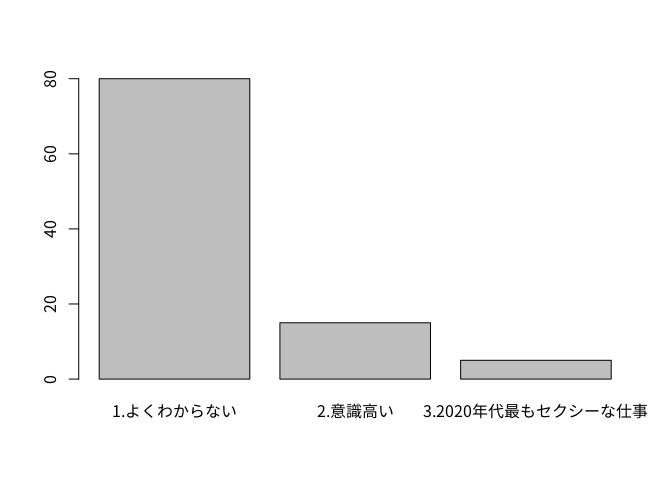
\includegraphics{Presentation_files/figure-beamer/unnamed-chunk-1-1.pdf}

\end{frame}

\begin{frame}{きぬいともよくわかんない}

\begin{itemize}
\tightlist
\item
  「ドリルを買う人は、ドリルがほしいんじゃなくて、穴がほしいんだよ」
\end{itemize}

\begin{itemize}
\tightlist
\item
  新人だったころのきぬいと「胡散臭い」
\end{itemize}

\end{frame}

\begin{frame}{「マーケティング」のよくわからなさ}

\begin{itemize}
\tightlist
\item
  どうなったら「うまくいった」と言えるのかがよくわからない

  \begin{itemize}
  \tightlist
  \item
    測定指標(KGIだのKPIだの)の定義がTPOによって異なる

    \begin{itemize}
    \tightlist
    \item
      あるいは大きく定義変更がなされる
    \end{itemize}
  \end{itemize}
\item
  指標の測定方法もよくわからない

  \begin{itemize}
  \tightlist
  \item
    この辺は実験計画法とか結構大事
  \item
    でもよくわからないまま実行しがち
  \end{itemize}
\item
  データ活用法のよくわからなさ

  \begin{itemize}
  \tightlist
  \item
    大体の日本企業はデータはある

    \begin{itemize}
    \tightlist
    \item
      「何がわかれば利益につながるのか」よくわからない
    \end{itemize}
  \item
    選択肢が多すぎると逆に選べない
  \item
    どんなデータがあると何がわかるのかよくわからない
  \end{itemize}
\end{itemize}

\end{frame}

\begin{frame}{}
\protect\hypertarget{section}{}

なんもわからん

\includegraphics{./.picture/erudesusono2.jpg}

\end{frame}

\section{データは使いたい}

\section{でもデータ活用は進まない}

\begin{frame}{}
\protect\hypertarget{section-1}{}

Just You Know Why

\includegraphics{./.picture/justyouknowwhy.jpg}

\begin{itemize}
\tightlist
\item
  知らない人は「panda チーズ」でググって
\end{itemize}

\end{frame}

\hypertarget{1.-kkd}{%
\section{理由1. KKD信仰}\label{1.-kkd}}

\begin{frame}{KKD(経験・勘・度胸)}
\protect\hypertarget{kkd}{}

\begin{itemize}
\tightlist
\item
  実際その道のベテランのK・Kは馬鹿にはできない(くやしい)

  \begin{itemize}
  \tightlist
  \item
    実際Dなしに決定はできない(それはそう)
  \end{itemize}
\item
  データ分析の価値もKKDに合うかどうかで決まるところもある

  \begin{itemize}
  \tightlist
  \item
    「合っているかどうか」を評価する基準が定義できない\\
  \item
    結果「経験」「勘」に頼らざるを得ない
  \end{itemize}
\end{itemize}

\end{frame}

\hypertarget{2.-excel}{%
\section{理由2. Excel信仰}\label{2.-excel}}

\hypertarget{excel}{%
\section{「Excelでできるじゃん」}\label{excel}}

\section{反論できず悔しい}

\section{わかる}

\begin{frame}{「Excelでなんでもできるじゃん」}
\protect\hypertarget{excel}{}

\begin{itemize}
\tightlist
\item
  「なんでもはできないわよ、できることだけ」

  \begin{itemize}
  \tightlist
  \item
    Excelでの手計算のミスが業務の8割を占めた2018年度
  \item
    誰もやりたくてやらかすわけじゃない
  \end{itemize}
\item
  「できる」から「効率化」へ

  \begin{itemize}
  \tightlist
  \item
    「Excelでできる」は「最適解」とは限らない

    \begin{itemize}
    \tightlist
    \item
      ちょっと仕様が変わると詰みがちなVBA
    \item
      エンジニアリングしなくても実装できる関数
    \item
      進まないバージョン管理
    \end{itemize}
  \end{itemize}
\end{itemize}

\end{frame}

\begin{frame}{その結果}

\begin{itemize}
\tightlist
\item
  【きぬいと編集】案件結果\_上司確認\_ver2\_2019xxxx.xls
\end{itemize}

\includegraphics{./.picture/chanmio.jpg}

\end{frame}

\hypertarget{tech}{%
\section{非Tech系データ分析}\label{tech}}

\begin{frame}[fragile]{仕事の8割が記述統計}
\protect\hypertarget{8}{}

\begin{itemize}
\tightlist
\item
  \texttt{table}や\texttt{ggplot}で解決する問題が大半

  \begin{itemize}
  \tightlist
  \item
    そもそも誰もデータを見ていない

    \begin{itemize}
    \tightlist
    \item
      故にKPIもKGIもよくわからない
    \end{itemize}
  \item
    分布や単純なクロス集計だけでも発見があることが多い

    \begin{itemize}
    \tightlist
    \item
      ここで初めてどの指標の評価をするかも判断できる
    \end{itemize}
  \end{itemize}
\item
  予測や分類はこの次のステップ

  \begin{itemize}
  \tightlist
  \item
    データをちゃんと見せよう
  \item
    魅せることすら時期尚早
  \end{itemize}
\end{itemize}

\end{frame}

\begin{frame}[fragile]{非Tech的Rの記述}
\protect\hypertarget{techr}{}

\begin{itemize}
\tightlist
\item
  記述統計レベルで解決する場合が多い

  \begin{itemize}
  \tightlist
  \item
    と言いつつそこそこデータ量が多い
  \end{itemize}
\item
  ある業務でのきぬいと
\end{itemize}

\begin{Shaded}
\begin{Highlighting}[]
\NormalTok{  dat <-}\StringTok{ }\NormalTok{datA }\OperatorTok\StringTok{ }
\StringTok{    }\NormalTok{dplyr}\OperatorTok{::}\KeywordTok{group_by}\NormalTok{(ID, date) }\OperatorTok\StringTok{ }
\StringTok{    }\NormalTok{dplyr}\OperatorTok{::}\KeywordTok{summarise}\NormalTok{(}\DataTypeTok{count =} \KeywordTok{n}\NormalTok{()) }\OperatorTok\StringTok{ }
\StringTok{    }\NormalTok{tidyr}\OperatorTok{::}\KeywordTok{spread}\NormalTok{(.,}\DataTypeTok{key =}\NormalTok{ date, }\DataTypeTok{value =}\NormalTok{ count) }\OperatorTok\StringTok{ }
\StringTok{    }\NormalTok{dplyr}\OperatorTok{::}\KeywordTok{mutate_if}\NormalTok{(is.numeric, }\KeywordTok{funs}\NormalTok{(}\KeywordTok{replace}\NormalTok{(.,}\KeywordTok{is.na}\NormalTok{(.),}\DecValTok{0}\NormalTok{))) }\OperatorTok\StringTok{ }
\StringTok{    }\NormalTok{dplyr}\OperatorTok{::}\KeywordTok{ungroup}\NormalTok{()}
\end{Highlighting}
\end{Shaded}

\begin{itemize}
\tightlist
\item
  これでログ形式のデータからIDと時系列別に何かをカウントして横展開とかする

  \begin{itemize}
  \tightlist
  \item
    そして平均とか行和列和とか見ながらグラフ出すとか
  \end{itemize}
\end{itemize}

\end{frame}

\begin{frame}[fragile]{出力}

\begin{Shaded}
\begin{Highlighting}[]
\NormalTok{dat[,}\DecValTok{1}\OperatorTok{:}\DecValTok{10}\NormalTok{] }\OperatorTok\StringTok{ }\NormalTok{head}
\end{Highlighting}
\end{Shaded}

\begin{verbatim}
## # A tibble: 6 x 10
##      ID `100` `101` `102` `103` `104` `105` `106` `107` `108`
##   <int> <dbl> <dbl> <dbl> <dbl> <dbl> <dbl> <dbl> <dbl> <dbl>
## 1     1     1     0     0     0     0     0     0     0     0
## 2     2     0     1     0     0     0     0     0     0     0
## 3     3     0     0     1     0     0     0     0     0     0
## 4     4     0     0     0     1     0     0     0     0     0
## 5     5     0     0     0     0     1     0     0     0     0
## 6     6     0     0     0     0     0     1     0     0     0
\end{verbatim}

\end{frame}

\begin{frame}{つまり?}

\begin{block}{整 然 宇 宙 開 発 局}

\includegraphics{./.picture/tidyverse.png}

\end{block}

\end{frame}

\begin{frame}[fragile]{冗談抜きで}

\begin{itemize}
\tightlist
\item
  \texttt{tidyverse}で既存業務がだいぶ改善した

  \begin{itemize}
  \tightlist
  \item
    残業時間を大幅に減らしたらストレスが減った
  \item
    上司が助かっているかはわからない\ldots{}\ldots{}助かっていると信じたい
  \end{itemize}
\item
  でかいExcelファイルを開くのに待つ必要性がだいぶ減った
\item
  \texttt{ggplot2}やら\texttt{DiagrammeR}やらでの可視化で表を見やすくできる
\item
  いいぞ
\end{itemize}

\end{frame}

\begin{frame}{お客様の声}

\begin{itemize}
\tightlist
\item
  「この動きは知らなかったなあ」
\item
  「ライバルと比べるとこうなっているのか」
\item
  「ここからこういうことできますか?」
\end{itemize}

\end{frame}

\begin{frame}{結論}

\begin{itemize}
\tightlist
\item
  Marketing Scienceは記述統計から入ろう

  \begin{itemize}
  \tightlist
  \item
    回帰分析とか誰も知らない
  \item
    よくあるご質問「切片は誤差ですか?」
  \end{itemize}
\item
  Statisticの語源に忠実にいこう

  \begin{itemize}
  \tightlist
  \item
    state/status「状態」の記述
  \item
    マーケティングで推定とかそんなの魔法っすよ。
  \end{itemize}
\end{itemize}

\end{frame}

\begin{frame}{今後}

\begin{itemize}
\tightlist
\item
  研修とかのためにこれまでのTipsをドキュメント化する

  \begin{itemize}
  \tightlist
  \item
    Rmdでいけんじゃね?

    \begin{itemize}
    \tightlist
    \item
      たまにPython使うけど
    \item
      PythonもRmdでまとめられるんじゃね?
    \end{itemize}
  \end{itemize}
\item
  R開発環境の統一

  \begin{itemize}
  \tightlist
  \item
    バージョン管理がめんどい

    \begin{itemize}
    \tightlist
    \item
      未だに社員のローカル環境依存
    \item
      こんな課題を解決したい(エンジニア発想)
    \end{itemize}
  \item
    Docker使えばなんとかなんじゃね?
  \item
    鋭意開発中

    \begin{itemize}
    \tightlist
    \item
      この辺知ってて一緒に働きたい人も募集中
    \end{itemize}
  \end{itemize}
\end{itemize}

\end{frame}

\hypertarget{enjoy}{%
\section{Enjoy!!}\label{enjoy}}

\end{document}
